Creating the bathymetries for the model was done using bathymetries from Muller et al.\cite{Muller2008Mar} these were scaled to a 4 degree model and subsequently changed to address passage openings in the 4 degree case where, due to the low resolution of the model, choices have to be made with respect to the opening of certain passages. One of the choices that was made specifically is to change the bathymetry of the standard 4 degree model to a custom one made in the same process as the other bathymetries too more accurately portray changes that occur using this process. One of the choices that was made is that the northern Sea is closed of in all of the bathymetries. This is mainly due to the fact that 4 degree models do not have enough resolution to support This sea and can cause strange behaviour to occur. Also there is little connection to the other oceans, thus negating the need for such a basin to be in our model.

The main events that shape the oceanic passages can be devided into time periods. These time periods are defined as follows in this paper. This deviates from their definitions in literature but serves only as a means of applying a name to the time steps.

\begin{table}[H]
	\begin{tabular}{lll}
		&From &Until \\
		Paleocene & 65Ma&55Ma    \\
		Eocene    & 50Ma&35Ma     \\
		Oligocene & 30Ma&20Ma    \\
		Miocene   & 20Ma&Present 
	\end{tabular}
\end{table}

%TODO (Relevant figures from paleoscene showing changes)
The model is started in the Paleocene where in the beginning a vast Pacific exists almost serving as a single basin. This period is largely characterized by the growth and development of a larger atlantic basin. Serving to decrease the size of the pacific basin. This can be seen in Figure %TODO add figures showing diffirence in size. 
Where the changes during the paleoscene are shown.
\begin{figure}[H]
	
	
	\centering
	\begin{subfigure}[b]{\linewidth}
		\centering
		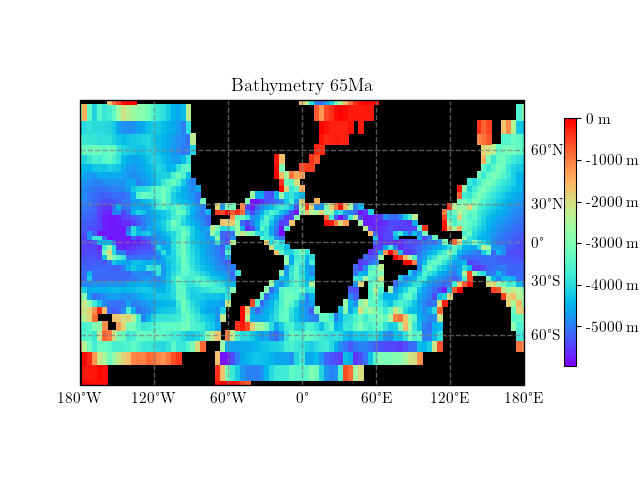
\includegraphics[width=\linewidth]{bathymetry/baath_65.png}
		\caption{Beginning of the Paleocene}
	\end{subfigure}
\begin{subfigure}[b]{\linewidth}
	\centering
	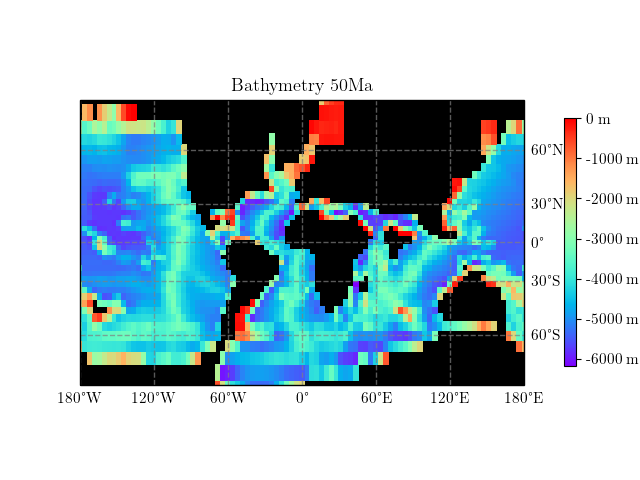
\includegraphics[width=\linewidth]{bathymetry/baath_50.png}
	\caption{End of the Paleocene}
\end{subfigure}
	\caption{}
	\label{fig:paleocene_bath}
\end{figure}


%TODO Eocene Drake-indian-tasman passages + depth

The Eocene in contrast to the Paleocene is destinguised by The opening of certain passages connecting oceanic basins. These effects are often studied extensively for each individual passage. Choosing the exact timespan for opening the passages is done manualy by looking at often active research takin into account big uncertaincies in the exact timing of the openings. The Eocene is characterized by several large events shown in Figure %todo add figure showing the events in detail
The first of such events that occurs is the indian continent colliding with the eurasian continent This has the effect of closing the deep water formations between the Thetys sea and the Indian ocean.
Next the Tasman passage is opened\cite{Lawver2003Sep} as a shallow passage slowly growing in size. The tasman passage opening is believed to have had a large impact on the onset of the ACC. The Total circulation of water around the antartic basin is finalized by the opening of the shallow Drake passage some 30Ma. 30Ma is specifically chosen to diffirentiate between the diffirent passage openings. Especially since there is still ongoing debate on the exact timing of drake passage opening.
%30ma drake passage opening (chosen as to diffirentiate between diffirent stages)
%35ma Indian passage closure
%35ma Tasman passage opening
%Indian continent colliding

%TODO Oligocene changes
The next time period is the oligocene Which is largely characterized by the deepening of the Tasman and drake passage and further expansion of the atlantic basin. It is believed %source
That the onset of the northern sinking atlantic started in this time period. Also the ACC probably is increasing in strenght.


%TODO Miocene

The miocene is Characterized by yet more increase in strenght of the ACC. Also Some more passage closures occur. Starting with the closure of the Thetys Seaway which had been decreasing in size in the previous 20Ma. Also the passage between modern day australia and indonesia is significantly decreasing in size due to the onset  of multiple vulcanic islands making the passage more narrow and shallow. Showing especially in this model. Further more the Thethys gateway
%0Ma current
%5Ma Wider Indonesia
%10ma last CAS
%14ma Thetys seaway last open 15ma first occurrence



Drake passage opening \cite{Scher2006Apr}

Tasman passage opening 

Central American seaway closure \cite{Molnar2008Jun} (deepwater 7Ma (10 for paper))\cite{Pindell1988Dec}

Tethys seaway closure \cite{Hamon2013Nov}

Widening of indonsian seaway (due to australia moving up.)


titis passage opening 

Choises made. 

Examples of where these choises interfere with reality.

Individual passages.

What age are we dealing with (Events/Changes observed in literature)

